\documentclass[a4paper,landscape]{article}
\usepackage[top=0.6cm,bottom=0.6cm,left=0.6cm,right=0.6cm,landscape]{geometry}
\usepackage{tikz}
\usetikzlibrary{arrows.meta,backgrounds,fit,calc}
\usepackage{xcolor}
\usepackage[T1]{fontenc}
\usepackage[utf8]{inputenc}
\usepackage{lmodern}
\usepackage{amsmath}
\usepackage{multicol}
\usepackage{enumitem}
\usepackage[most]{tcolorbox}
\usepackage{parskip}
\usepackage{booktabs}
\usepackage{multirow}
\usepackage{mdframed}

% ── Boîtes colorées réutilisables ─────────────────────────────────────
\tcbuselibrary{skins,breakable}
\newtcolorbox{defbox}[2][]{
    colback=#2!8, colframe=#2, fonttitle=\bfseries\small,
    title={#1}, arc=4pt, boxrule=1.2pt, left=6pt, right=6pt,
    top=4pt, bottom=4pt, #1
}
\newtcolorbox{stepbox}[2][]{
    colback=white, colframe=#2, fonttitle=\bfseries\small\color{white},
    attach boxed title to top left={yshift=-2mm,xshift=6pt},
    boxed title style={colback=#2,arc=3pt,boxrule=0pt},
    title={#1}, arc=4pt, boxrule=1.0pt, left=6pt, right=6pt,
    top=8pt, bottom=4pt
}

\definecolor{colServer} {RGB}{41,128,185}
\definecolor{colAgent}  {RGB}{39,174,96}
\definecolor{colTrainer}{RGB}{142,68,173}
\definecolor{colTopic}  {RGB}{231,76,60}
\definecolor{colNN}     {RGB}{243,156,18}
\definecolor{colROS}    {RGB}{52,73,94}
\definecolor{colBG}     {RGB}{245,247,250}
\definecolor{colEp}     {RGB}{22,160,133}

\begin{document}
\pagestyle{empty}

% ═══════════════════════════════════════════════════════════════════════
%  PAGE 1 — ARCHITECTURE SYSTÈME GLOBALE
%  Layout : agents en rangée horizontale, buses horizontaux
%  → aucun croisement possible
% ═══════════════════════════════════════════════════════════════════════
\noindent
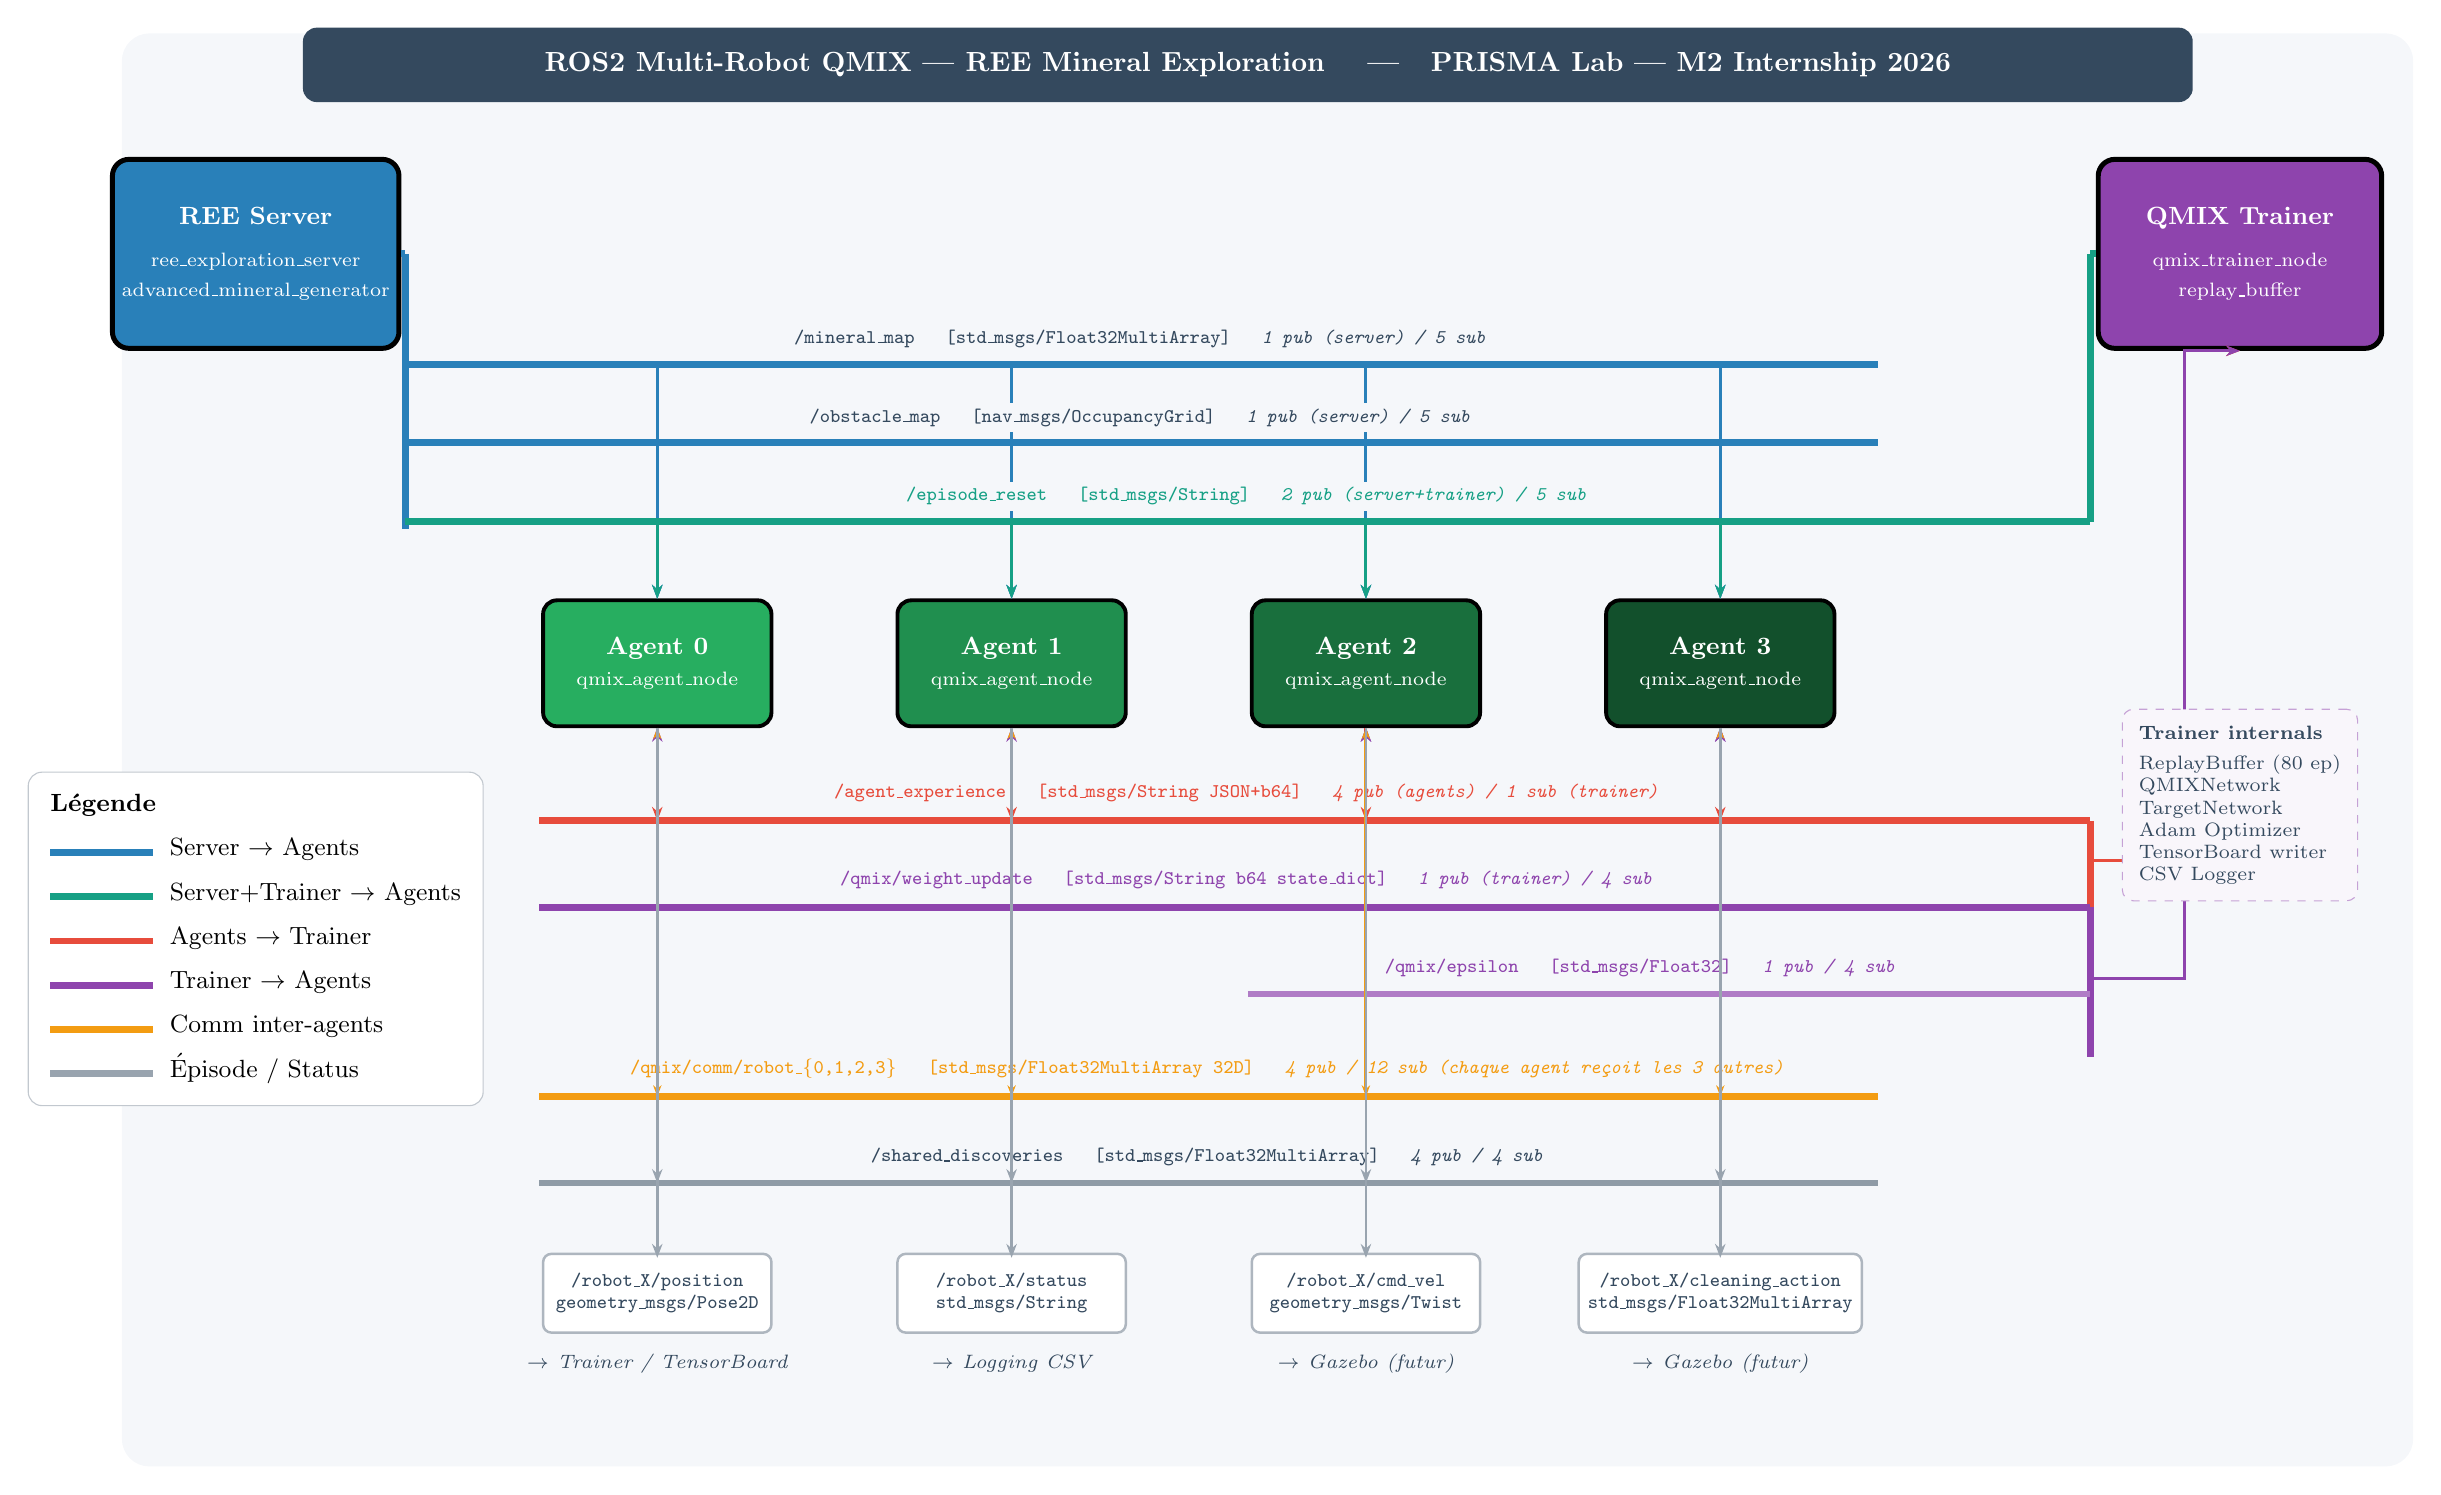
\begin{tikzpicture}[
    every node/.style={font=\small},
    % ── nœuds principaux ──────────────────────────────────────────────
    mainNode/.style ={rectangle,rounded corners=6pt,align=center,
                      text=white,draw,line width=1.8pt,
                      minimum width=3.6cm,minimum height=2.4cm},
    agentNode/.style={rectangle,rounded corners=5pt,align=center,
                      text=white,draw,line width=1.4pt,
                      minimum width=2.9cm,minimum height=1.6cm},
    statusBox/.style={rectangle,rounded corners=3pt,align=center,
                      fill=white,draw=colROS!40,line width=0.9pt,
                      font=\scriptsize\ttfamily,text=colROS,
                      minimum width=2.9cm,minimum height=1.0cm},
    % ── étiquettes de bus ─────────────────────────────────────────────
    busLbl/.style   ={font=\scriptsize\ttfamily,fill=colBG,
                      inner sep=2pt,text=colROS},
    % ── flèches ───────────────────────────────────────────────────────
    dropS/.style ={-{Stealth[length=5pt]},colServer, line width=1.1pt},
    dropT/.style ={-{Stealth[length=5pt]},colTrainer,line width=1.1pt},
    dropR/.style ={-{Stealth[length=5pt]},colTopic,  line width=1.1pt},
    dropE/.style ={-{Stealth[length=5pt]},colEp,     line width=1.1pt},
    dropG/.style ={-{Stealth[length=5pt]},colROS!50, line width=1.0pt},
    biN/.style   ={{Stealth[length=4pt]}-{Stealth[length=4pt]},
                   colNN,line width=1.1pt},
]

%─── FOND ──────────────────────────────────────────────────────────────
\fill[colBG,rounded corners=10pt] (-0.3,-10.2) rectangle (28.8,8.0);

%─── BARRE TITRE ───────────────────────────────────────────────────────
\node[fill=colROS,text=white,rounded corners=5pt,
      font=\normalsize\bfseries,inner sep=9pt,minimum width=24cm]
      at (14.0,7.6)
      {ROS2 Multi-Robot QMIX \textbf{---} REE Mineral Exploration
       \quad|\quad PRISMA Lab --- M2 Internship 2026};

%─── SERVER ────────────────────────────────────────────────────────────
\node[mainNode,fill=colServer] (server) at (1.4,5.2)
    {\textbf{REE Server}\\[4pt]
     \scriptsize ree\_exploration\_server\\
     \scriptsize advanced\_mineral\_generator};

%─── TRAINER ───────────────────────────────────────────────────────────
\node[mainNode,fill=colTrainer] (trainer) at (26.6,5.2)
    {\textbf{QMIX Trainer}\\[4pt]
     \scriptsize qmix\_trainer\_node\\
     \scriptsize replay\_buffer};

%─── AGENTS (rangée horizontale, même y=0) ─────────────────────────────
\def\Apos{ {6.5}, {11.0}, {15.5}, {20.0} }

\node[agentNode,fill=colAgent]           (a0) at ( 6.5,0)
    {\textbf{Agent 0}\\\scriptsize qmix\_agent\_node};
\node[agentNode,fill=colAgent!82!black]  (a1) at (11.0,0)
    {\textbf{Agent 1}\\\scriptsize qmix\_agent\_node};
\node[agentNode,fill=colAgent!64!black]  (a2) at (15.5,0)
    {\textbf{Agent 2}\\\scriptsize qmix\_agent\_node};
\node[agentNode,fill=colAgent!46!black]  (a3) at (20.0,0)
    {\textbf{Agent 3}\\\scriptsize qmix\_agent\_node};

\begin{scope}[on background layer]
\node[draw=colAgent,dashed,line width=1.2pt,rounded corners=8pt,
      fill=colAgent!5,fit=(a0)(a1)(a2)(a3),inner sep=10pt,
      label={[font=\small\bfseries,text=colAgent,yshift=4pt]above:%
             4 Agents QMIX --- Exécution Décentralisée}]
      (agGroup){};
\end{scope}

% ═══════════════════════════════════════════════════════════════════════
%  SECTION 1 : SERVEUR → AGENTS
%  Colonne vertébrale du serveur à x=3.3 (juste à droite du serveur)
%  Trois buses horizontaux, flèches verticales vers chaque agent
% ═══════════════════════════════════════════════════════════════════════

% Colonne vertébrale serveur
\draw[colServer,line width=2.5pt] (server.east) -- (3.3,5.2);
\draw[colServer,line width=2.5pt] (3.3,5.2)    -- (3.3,1.7);

%── Bus /mineral_map  (y=3.8) ─────────────────────────────────────────
\draw[colServer,line width=2.5pt] (3.3,3.8) -- (22.0,3.8);
\node[busLbl] at (12.65,4.12)
    {\textbf{/mineral\_map} \quad [std\_msgs/Float32MultiArray] \quad
     \textit{1 pub (server) / 5 sub}};
\foreach \ax in {6.5,11.0,15.5,20.0}
    \draw[dropS] (\ax,3.8) -- (\ax,0.82);

%── Bus /obstacle_map (y=2.8) ─────────────────────────────────────────
\draw[colServer,line width=2.5pt] (3.3,2.8) -- (22.0,2.8);
\node[busLbl] at (12.65,3.12)
    {\textbf{/obstacle\_map} \quad [nav\_msgs/OccupancyGrid] \quad
     \textit{1 pub (server) / 5 sub}};
\foreach \ax in {6.5,11.0,15.5,20.0}
    \draw[dropS] (\ax,2.8) -- (\ax,0.82);

%── Bus /episode_reset (y=1.8) — Server ET Trainer publient ───────────
\draw[colEp,line width=2.5pt] (3.3,1.8) -- (24.7,1.8);
\node[busLbl,text=colEp] at (14.0,2.12)
    {\textbf{/episode\_reset} \quad [std\_msgs/String] \quad
     \textit{2 pub (server+trainer) / 5 sub}};
\foreach \ax in {6.5,11.0,15.5,20.0}
    \draw[dropE] (\ax,1.8) -- (\ax,0.82);

% Trainer → /episode_reset (colonne vertébrale trainer à droite)
\draw[colEp,line width=2.5pt] (trainer.west) -- (24.7,5.2);
\draw[colEp,line width=2.5pt] (24.7,5.2)    -- (24.7,1.8);

% ═══════════════════════════════════════════════════════════════════════
%  SECTION 2 : AGENTS → TRAINER
%  Buses horizontaux sous les agents, flèches verticales montantes
% ═══════════════════════════════════════════════════════════════════════

%── Bus /agent_experience (y=-2.0) ────────────────────────────────────
\draw[colTopic,line width=2.5pt] (5.0,-2.0) -- (24.7,-2.0);
\node[busLbl,text=colTopic] at (14.0,-1.65)
    {\textbf{/agent\_experience} \quad [std\_msgs/String JSON+b64] \quad
     \textit{4 pub (agents) / 1 sub (trainer)}};
\foreach \ax in {6.5,11.0,15.5,20.0}
    \draw[dropR] (\ax,-0.82) -- (\ax,-2.0);
% Bus → Trainer (via colonne vertébrale trainer)
\draw[colTopic,line width=2.5pt] (24.7,-2.0) -- (24.7,-5.0);
\draw[dropR] (24.7,-2.5) -- ++(1.2,0) |- (trainer.south);

%── Bus /qmix/weight_update (y=-3.1) ──────────────────────────────────
\draw[colTrainer,line width=2.5pt] (5.0,-3.1) -- (24.7,-3.1);
\node[busLbl,text=colTrainer] at (14.0,-2.75)
    {\textbf{/qmix/weight\_update} \quad [std\_msgs/String b64 state\_dict] \quad
     \textit{1 pub (trainer) / 4 sub}};
% Trainer → bus (colonne vertébrale)
\draw[colTrainer,line width=2.5pt] (24.7,-3.1) -- (24.7,-5.0);
\draw[dropT] (24.7,-4.0) -- ++(1.2,0) |- (trainer.south);
\foreach \ax in {6.5,11.0,15.5,20.0}
    \draw[dropT] (\ax,-3.1) -- (\ax,-0.82);

%── Bus /qmix/epsilon (y=-4.2 — agents 2 et 3 uniquement) ────────────
\draw[colTrainer!70,line width=2.5pt] (14.0,-4.2) -- (24.7,-4.2);
\node[busLbl,text=colTrainer] at (19.0,-3.87)
    {\textbf{/qmix/epsilon} \quad [std\_msgs/Float32] \quad
     \textit{1 pub / 4 sub}};
\foreach \ax in {15.5,20.0}
    \draw[dropT] (\ax,-4.2) -- (\ax,-0.82);

% ═══════════════════════════════════════════════════════════════════════
%  SECTION 3 : COMMUNICATION INTER-AGENTS
% ═══════════════════════════════════════════════════════════════════════

%── Bus /qmix/comm/robot_{0..3} (y=-5.5) ─────────────────────────────
\draw[colNN,line width=2.5pt] (5.0,-5.5) -- (22.0,-5.5);
\node[busLbl,text=colNN] at (13.5,-5.15)
    {\textbf{/qmix/comm/robot\_\{0,1,2,3\}} \quad
     [std\_msgs/Float32MultiArray 32D] \quad
     \textit{4 pub / 12 sub (chaque agent reçoit les 3 autres)}};
\foreach \ax in {6.5,11.0,15.5,20.0}
    \draw[biN] (\ax,-0.82) -- (\ax,-5.5);

%── Bus /shared_discoveries (y=-6.6) ──────────────────────────────────
\draw[colROS!55,line width=2.5pt] (5.0,-6.6) -- (22.0,-6.6);
\node[busLbl,text=colROS] at (13.5,-6.27)
    {\textbf{/shared\_discoveries} \quad [std\_msgs/Float32MultiArray] \quad
     \textit{4 pub / 4 sub}};
\foreach \ax in {6.5,11.0,15.5,20.0}
    \draw[dropG] (\ax,-0.82) -- (\ax,-6.6);

% ═══════════════════════════════════════════════════════════════════════
%  SECTION 4 : TOPICS STATUS ROBOTS (bas)
% ═══════════════════════════════════════════════════════════════════════

\node[statusBox] at ( 6.5,-8.0)
    {/robot\_X/\textbf{position}\\geometry\_msgs/Pose2D};
\node[statusBox] at (11.0,-8.0)
    {/robot\_X/\textbf{status}\\std\_msgs/String};
\node[statusBox] at (15.5,-8.0)
    {/robot\_X/\textbf{cmd\_vel}\\geometry\_msgs/Twist};
\node[statusBox] at (20.0,-8.0)
    {/robot\_X/\textbf{cleaning\_action}\\std\_msgs/Float32MultiArray};

\foreach \ax in {6.5,11.0,15.5,20.0}
    \draw[dropG] (\ax,-0.82) -- (\ax,-7.55);

\node[font=\scriptsize\itshape,text=colROS] at ( 6.5,-8.9) {$\to$ Trainer / TensorBoard};
\node[font=\scriptsize\itshape,text=colROS] at (11.0,-8.9) {$\to$ Logging CSV};
\node[font=\scriptsize\itshape,text=colROS] at (15.5,-8.9) {$\to$ Gazebo (futur)};
\node[font=\scriptsize\itshape,text=colROS] at (20.0,-8.9) {$\to$ Gazebo (futur)};

% ═══════════════════════════════════════════════════════════════════════
%  INTERNALS TRAINER
% ═══════════════════════════════════════════════════════════════════════

\node[draw=colTrainer!50,dashed,rounded corners=4pt,
      fill=colTrainer!5,align=left,
      font=\scriptsize,text=colROS,inner sep=6pt]
      (tInt) at (26.6,-1.8)
      {\textbf{Trainer internals}\\[3pt]
       ReplayBuffer (80 ep)\\
       QMIXNetwork\\
       TargetNetwork\\
       Adam Optimizer\\
       TensorBoard writer\\
       CSV Logger};

% ═══════════════════════════════════════════════════════════════════════
%  LÉGENDE
% ═══════════════════════════════════════════════════════════════════════

\node[draw=colROS!30,fill=white,rounded corners=5pt,
      align=left,font=\small,inner sep=8pt]
      at (1.4,-3.5)
      {\textbf{Légende}\\[5pt]
       \textcolor{colServer} {\rule{1.3cm}{2.5pt}}\ \ Server $\to$ Agents\\[5pt]
       \textcolor{colEp}     {\rule{1.3cm}{2.5pt}}\ \ Server+Trainer $\to$ Agents\\[5pt]
       \textcolor{colTopic}  {\rule{1.3cm}{2.5pt}}\ \ Agents $\to$ Trainer\\[5pt]
       \textcolor{colTrainer}{\rule{1.3cm}{2.5pt}}\ \ Trainer $\to$ Agents\\[5pt]
       \textcolor{colNN}     {\rule{1.3cm}{2.5pt}}\ \ Comm inter-agents\\[5pt]
       \textcolor{colROS!50} {\rule{1.3cm}{2.5pt}}\ \ Épisode / Status};

\end{tikzpicture}

% ═══════════════════════════════════════════════════════════════════════
%  PAGE 2 — PIPELINE INTERNE AGENT
% ═══════════════════════════════════════════════════════════════════════
\newpage
\noindent
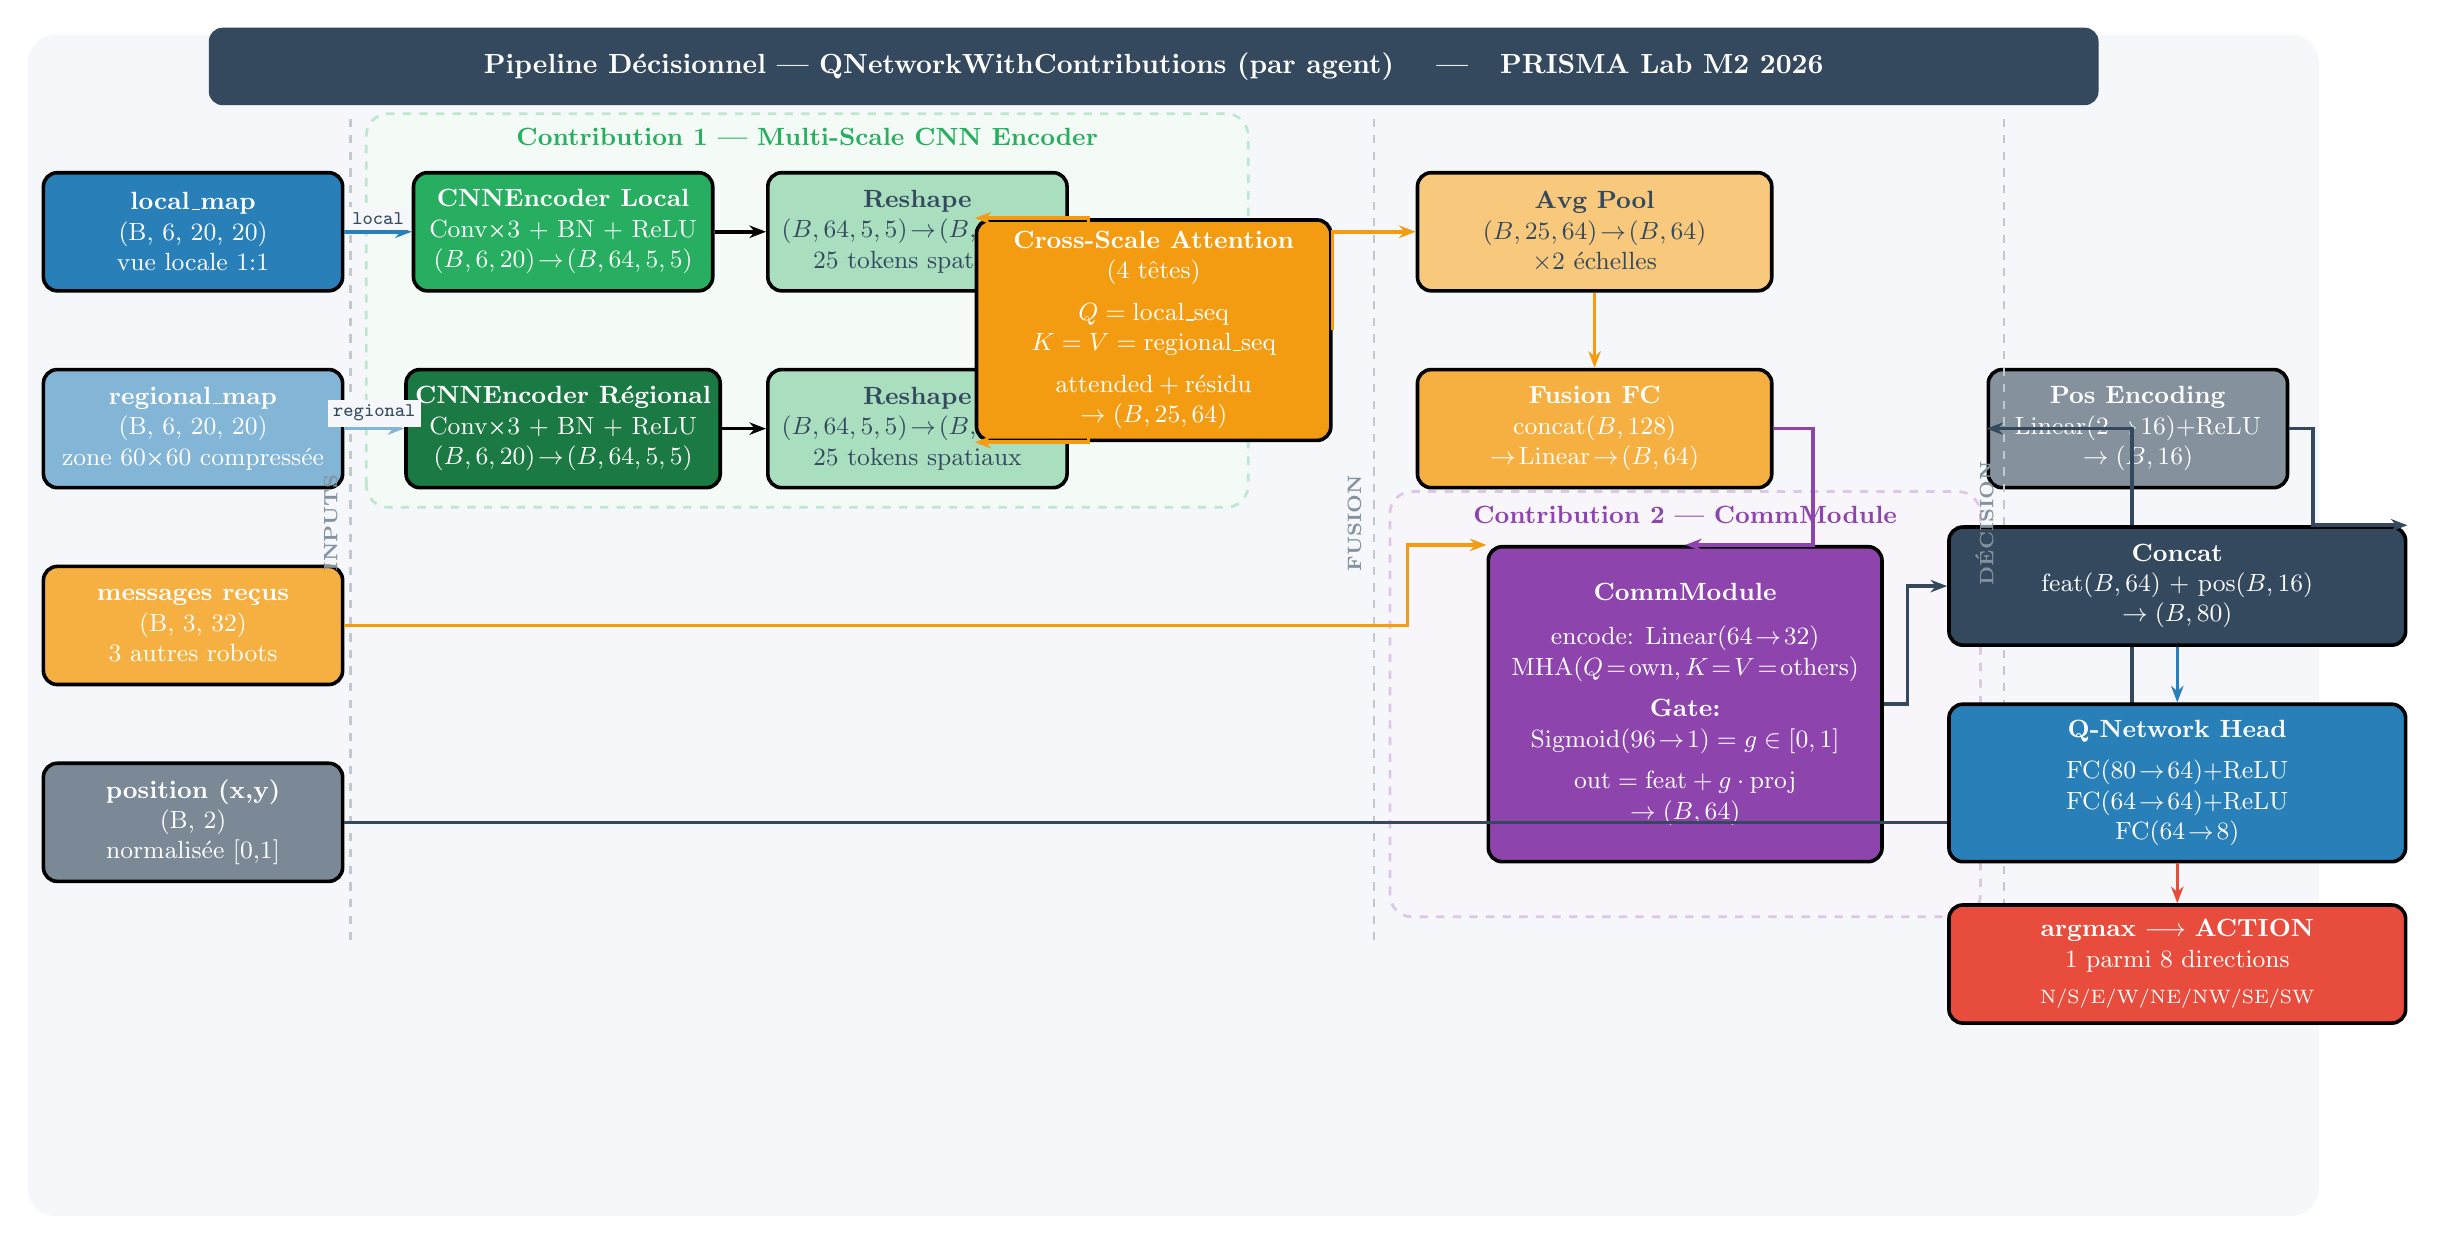
\begin{tikzpicture}[
    every node/.style={font=\small},
    blk/.style={rectangle,rounded corners=5pt,align=center,
                draw,line width=1.3pt,minimum width=3.8cm,
                minimum height=1.5cm},
    arr/.style={-{Stealth[length=6pt]},line width=1.3pt},
    lbl/.style={font=\scriptsize\ttfamily,fill=colBG,inner sep=2pt,text=colROS},
]

\fill[colBG,rounded corners=10pt] (-0.3,-7.0) rectangle (28.8,8.0);

%── BARRE TITRE ────────────────────────────────────────────────────────
\node[fill=colROS,text=white,rounded corners=5pt,
      font=\normalsize\bfseries,inner sep=9pt,minimum width=24cm]
      at (14.0,7.6)
      {Pipeline Décisionnel --- QNetworkWithContributions (par agent)
       \quad|\quad PRISMA Lab M2 2026};

%──────────────────────────────────────────────────────────────────────
%  INPUTS (colonne verticale de gauche)
%──────────────────────────────────────────────────────────────────────
\node[blk,fill=colServer,text=white]      (lIn)  at (1.8, 5.5)
    {\textbf{local\_map}\\(B,\ 6,\ 20,\ 20)\\vue locale 1:1};

\node[blk,fill=colServer!58,text=white]   (rIn)  at (1.8, 3.0)
    {\textbf{regional\_map}\\(B,\ 6,\ 20,\ 20)\\zone 60×60 compressée};

\node[blk,fill=colNN!80,text=white]       (cIn)  at (1.8, 0.5)
    {\textbf{messages reçus}\\(B,\ 3,\ 32)\\3 autres robots};

\node[blk,fill=colROS!65,text=white]      (pIn)  at (1.8,-2.0)
    {\textbf{position (x,y)}\\(B,\ 2)\\normalisée [0,1]};

% Séparateur inputs
\draw[colROS!30,dashed,line width=0.8pt] (3.8,-3.5) -- (3.8,7.0);
\node[font=\scriptsize\bfseries,text=colROS!60,rotate=90] at (3.55,1.8) {INPUTS};

%──────────────────────────────────────────────────────────────────────
%  CONTRIBUTION 1 : MULTI-SCALE CNN ENCODER
%──────────────────────────────────────────────────────────────────────
\draw[colAgent!30,fill=colAgent!5,rounded corners=8pt,line width=1.0pt,dashed]
    (4.0,2.0) rectangle (15.2,7.0);
\node[font=\small\bfseries,text=colAgent] at (9.6,6.7)
    {Contribution 1 — Multi-Scale CNN Encoder};

\node[blk,fill=colAgent,text=white]          (cnnL) at (6.5,5.5)
    {\textbf{CNNEncoder Local}\\Conv×3 + BN + ReLU\\$(B,6,20)\!\to\!(B,64,5,5)$};

\node[blk,fill=colAgent!70!black,text=white] (cnnR) at (6.5,3.0)
    {\textbf{CNNEncoder Régional}\\Conv×3 + BN + ReLU\\$(B,6,20)\!\to\!(B,64,5,5)$};

\draw[arr,color=colServer]       (lIn.east) -- node[lbl,above]{\scriptsize local}  (cnnL.west);
\draw[arr,color=colServer!58]    (rIn.east) -- node[lbl,above]{\scriptsize regional} (cnnR.west);

\node[blk,fill=colAgent!40,text=colROS] (reshL) at (11.0,5.5)
    {\textbf{Reshape}\\$(B,64,5,5)\!\to\!(B,25,64)$\\25 tokens spatiaux};

\node[blk,fill=colAgent!40,text=colROS] (reshR) at (11.0,3.0)
    {\textbf{Reshape}\\$(B,64,5,5)\!\to\!(B,25,64)$\\25 tokens spatiaux};

\draw[arr] (cnnL.east) -- (reshL.west);
\draw[arr] (cnnR.east) -- (reshR.west);

\node[blk,fill=colNN,text=white,minimum width=4.5cm,minimum height=2.8cm]
    (attn) at (14.0,4.25)
    {\textbf{Cross-Scale Attention}\\(4 têtes)\\[4pt]
     $Q = \text{local\_seq}$\\
     $K = V = \text{regional\_seq}$\\[4pt]
     $\text{attended} + \text{résidu}$\\
     $\to (B,25,64)$};

\draw[arr,color=colNN] (reshL.east) -- ++(0.25,0) |- (attn.north west);
\draw[arr,color=colNN] (reshR.east) -- ++(0.25,0) |- (attn.south west);

% Séparateur
\draw[colROS!30,dashed,line width=0.8pt] (16.8,-3.5) -- (16.8,7.0);

%──────────────────────────────────────────────────────────────────────
%  GLOBAL AVERAGE POOL + FUSION
%──────────────────────────────────────────────────────────────────────
\node[blk,fill=colNN!55,text=colROS,minimum width=4.5cm]
    (pool) at (19.6,5.5)
    {\textbf{Avg Pool}\\$(B,25,64)\!\to\!(B,64)$\\$\times 2$ échelles};

\node[blk,fill=colNN!80,text=white,minimum width=4.5cm]
    (fuse) at (19.6,3.0)
    {\textbf{Fusion FC}\\$\text{concat}(B,128)$\\$\to\!\text{Linear}\!\to\!(B,64)$};

\draw[arr,color=colNN] (attn.east) |- (pool.west);
\draw[arr,color=colNN] (pool.south) -- (fuse.north);

%──────────────────────────────────────────────────────────────────────
%  CONTRIBUTION 2 : COMMMODULE
%──────────────────────────────────────────────────────────────────────
\draw[colTrainer!30,fill=colTrainer!5,rounded corners=8pt,
      line width=1.0pt,dashed]
      (17.0,-3.2) rectangle (24.5,2.2);
\node[font=\small\bfseries,text=colTrainer] at (20.75,1.9)
    {Contribution 2 — CommModule};

\node[blk,fill=colTrainer,text=white,minimum width=5.0cm,minimum height=4.0cm]
    (comm) at (20.75,0.0-0.5)
    {\textbf{CommModule}\\[5pt]
     encode: Linear$(64\!\to\!32)$\\
     MHA$(Q\!=\!\text{own},K\!=\!V\!=\!\text{others})$\\[4pt]
     \textbf{Gate:}\\
     Sigmoid$(96\!\to\!1)=g\in[0,1]$\\[4pt]
     $\text{out}=\text{feat}+g\cdot\text{proj}$\\
     $\to(B,64)$};

\draw[arr,color=colNN]      (cIn.east)  -- ++(13.5,0) |- (comm.north west);
\draw[arr,color=colTrainer] (fuse.east) -- ++(0.5,0)  |- (comm.north);

%──────────────────────────────────────────────────────────────────────
%  POSITION ENCODING
%──────────────────────────────────────────────────────────────────────
\node[blk,fill=colROS!60,text=white,minimum width=3.8cm]
    (posEnc) at (26.5,3.0)
    {\textbf{Pos Encoding}\\Linear$(2\!\to\!16)$+ReLU\\$\to(B,16)$};

\draw[arr,color=colROS] (pIn.east) -- ++(22.7,0) |- (posEnc.west);

%──────────────────────────────────────────────────────────────────────
%  CONCAT + Q-NETWORK + ACTION
%──────────────────────────────────────────────────────────────────────
\draw[colROS!30,dashed,line width=0.8pt] (24.8,-3.5) -- (24.8,7.0);

\node[blk,fill=colROS,text=white,minimum width=5.8cm]
    (cat) at (27.0,1.0)
    {\textbf{Concat}\\feat$(B,64)$ + pos$(B,16)$\\$\to(B,80)$};

\draw[arr,color=colROS] (comm.east)   -- ++(0.3,0) |- (cat.west);
\draw[arr,color=colROS] (posEnc.east) -- ++(0.3,0) |- (cat.north east);

\node[blk,fill=colServer,text=white,minimum width=5.8cm,minimum height=2.0cm]
    (qnet) at (27.0,-1.5)
    {\textbf{Q-Network Head}\\[4pt]
     FC$(80\!\to\!64)$+ReLU\\
     FC$(64\!\to\!64)$+ReLU\\
     FC$(64\!\to\!8)$};

\draw[arr,color=colServer] (cat.south) -- (qnet.north);

\node[blk,fill=colTopic,text=white,minimum width=5.8cm]
    (act) at (27.0,-3.8)
    {\textbf{argmax} $\longrightarrow$ \textbf{ACTION}\\
     1 parmi 8 directions\\[2pt]
     \scriptsize N/S/E/W/NE/NW/SE/SW};

\draw[arr,color=colTopic] (qnet.south) -- (act.north);

% Labels colonnes
\node[font=\scriptsize\bfseries,text=colROS!60,rotate=90] at (16.55,1.8)  {FUSION};
\node[font=\scriptsize\bfseries,text=colROS!60,rotate=90] at (24.55,1.8)  {DÉCISION};

\end{tikzpicture}


% ═══════════════════════════════════════════════════════════════════════
%  PAGE 3 — QMIX : EXPLICATION DÉBUTANT
% ═══════════════════════════════════════════════════════════════════════
\newpage
\newgeometry{top=1.4cm,bottom=1.4cm,left=1.8cm,right=1.8cm}
\pagestyle{empty}

\begin{center}
    {\Large\bfseries\color{colROS}
     Explication --- QMIX, Contribution~1 \& Contribution~2}\\[0.25cm]
    {\normalsize\itshape\color{colROS!70}
     Stage M2 --- PRISMA Lab 2026 \quad|\quad
     Apprentissage par renforcement multi-agent pour l'exploration REE}
\end{center}
\vspace{0.2cm}
\noindent\rule{\linewidth}{1.5pt}
\vspace{0.15cm}

\begin{multicols}{2}

% ─────────────────────────────────────────────────────────────────────
\begin{tcolorbox}[colback=colROS!6,colframe=colROS,
    fonttitle=\bfseries\normalsize,title=Partie 0 — Le problème à résoudre,
    arc=5pt,boxrule=1.3pt]
Imagine une grande carte \textbf{100\(\times\)100 cases}.
Des gisements de minéraux rares (REE) sont cachés un peu partout.
Tu as \textbf{4 robots} pour les trouver.

Chaque robot ne voit qu'une \textit{petite zone} autour de lui.
S'ils n'apprennent pas à coopérer, deux robots peuvent fouiller la même
zone pendant que l'autre moitié de la carte reste inexplorée.

\medskip
\textbf{Objectif :} apprendre aux robots à coopérer
\textit{sans programmer chaque décision à la main.}
\(\Rightarrow\) Solution : apprentissage par renforcement multi-agent \textbf{QMIX}.
\end{tcolorbox}

\vspace{0.35cm}

% ─────────────────────────────────────────────────────────────────────
\begin{tcolorbox}[colback=colServer!6,colframe=colServer,
    fonttitle=\bfseries\normalsize,title=Partie 1 — QMIX expliqué simplement,
    arc=5pt,boxrule=1.3pt]

\textbf{Apprentissage par renforcement (base)}

Un robot apprend comme un enfant avec des points :
essaie une action \(\to\) reçoit une récompense \(\to\) mémorise ce qui marche.
Le réseau de neurones apprend un \textbf{score Q} par action~:
\[
    Q(s,a) \;=\; \text{récompense espérée si on fait l'action } a \text{ depuis l'état } s
\]
L'action choisie = celle avec le score Q le plus élevé.

\medskip
\textbf{Le problème avec plusieurs agents}

Si 4 robots apprennent séparément, ils peuvent se gêner sans le savoir
(2 robots qui couvrent la même zone, 2 zones jamais visitées).
Il faut optimiser une \textit{récompense globale} d'équipe.

\medskip
\textbf{L'idée centrale de QMIX}

\begin{center}
\textit{«\,Si l'équipe gagne, chaque membre a bien joué.\,»}
\end{center}

QMIX apprend une valeur globale \(Q_{\text{tot}}\) et \textbf{garantit} :
\[
    \frac{\partial Q_{\text{tot}}}{\partial Q_i} \;\geq\; 0
    \quad \forall\, \text{robot } i
\]
Augmenter le score individuel d'un robot augmente toujours le score total.
C'est la propriété \textbf{IGM} (Individual-Global Max).

\medskip
\textbf{Architecture QMIX (CTDE)}

\begin{center}
\small
\begin{tabular}{@{}ll@{}}
\toprule
Entraînement & centralisé (accès à tout) \\
Exécution    & décentralisée (chaque robot seul) \\
\bottomrule
\end{tabular}
\end{center}

\medskip
\begin{itemize}[leftmargin=1.2em,itemsep=2pt]
    \item Chaque robot calcule ses Q-valeurs locales \(Q_i\)
    \item Le \textbf{Mixing Network} combine les \(Q_i\) en \(Q_{\text{tot}}\)
          en utilisant l'état global de la carte
    \item Les poids du Mixing Network sont toujours \(\geq 0\) (via
          \texttt{torch.abs}), garantissant la monotonie IGM
\end{itemize}

\medskip
\textbf{Ce que chaque robot voit — observation 20\(\times\)20\(\times\)6}

\begin{center}
\small
\begin{tabular}{@{}cl@{}}
\toprule
Canal & Contenu \\
\midrule
1 & Concentration REE\_Oxides \\
2 & Concentration REE\_Silicates \\
3 & Concentration REE\_Phosphates \\
4 & Concentration REE\_Carbonates \\
5 & Présence d'obstacles \\
6 & Cases déjà explorées \\
\bottomrule
\end{tabular}
\end{center}

\medskip
\textbf{Cycle d'apprentissage QMIX}

\begin{enumerate}[leftmargin=1.5em,itemsep=2pt]
    \item Les robots explorent et stockent leurs expériences
          (\textit{obs, action, récompense, obs suivante})
    \item Le trainer tire un batch du \textit{replay buffer}
    \item Calcule \(Q_i\) pour tous les agents \(\to\) mélange \(\to Q_{\text{tot}}\)
    \item Compare à \((r + \gamma \cdot Q_{\text{tot}}^{\text{cible}})\)
          et réduit l'erreur par rétropropagation
    \item Met à jour les poids partagés des 4 agents
\end{enumerate}

\end{tcolorbox}

\columnbreak

% ─────────────────────────────────────────────────────────────────────
\begin{tcolorbox}[colback=colAgent!6,colframe=colAgent,
    fonttitle=\bfseries\normalsize,
    title=Partie 2 — Contribution 1 : Multi-Scale CNN Encoder,
    arc=5pt,boxrule=1.3pt]

\textbf{Le problème}

Avec une observation 20\(\times\)20, le robot voit les détails immédiats
mais est \textit{aveugle} aux structures plus lointaines.
Un gisement à 30 cases peut passer inaperçu.

\medskip
\textbf{La solution : deux zooms simultanés}

\begin{itemize}[leftmargin=1.2em,itemsep=2pt]
    \item \textbf{Observation locale} : fenêtre 20\(\times\)20 à résolution 1:1
          \(\to\) détails fins autour du robot
    \item \textbf{Observation régionale} : fenêtre 60\(\times\)60 compressée
          à 20\(\times\)20 (average pooling \(\times3\))
          \(\to\) panorama large, moins précis
\end{itemize}

Chaque vue passe dans son propre \textbf{CNN} (3 convolutions + BatchNorm)
et produit \textbf{25 tokens spatiaux} de 64 dimensions chacun.

\medskip
\textbf{Cross-Scale Attention (la fusion intelligente)}

Le robot ne concatène pas bêtement les deux vues.
Il utilise l'attention pour demander : \textit{«\,quelle partie de
la vue régionale est utile pour chaque position locale~?\,»}

\[
Q = \text{tokens locaux},\quad
K = V = \text{tokens régionaux}
\]
\[
\text{attended} = \text{MultiheadAttention}(Q, K, V)
\]

Connexion résiduelle + LayerNorm \(\to\) stabilité de l'entraînement.

\medskip
\textbf{Résultat}

\begin{center}
\small
local (B,25,64) + régional (B,25,64)\\
\(\downarrow\) \textit{average pooling + concat + FC}\\
\(\mathbf{h_i}\) \textbf{(B, 64)} --- représentation riche multi-échelle
\end{center}

L'agent apprend à détecter une veine de minerais 3\(\times\) plus loin
et à orienter ses décisions locales en conséquence.

\end{tcolorbox}

\vspace{0.35cm}

% ─────────────────────────────────────────────────────────────────────
\begin{tcolorbox}[colback=colTrainer!6,colframe=colTrainer,
    fonttitle=\bfseries\normalsize,
    title=Partie 3 — Contribution 2 : GeoCommQMIX (Communication),
    arc=5pt,boxrule=1.3pt]

\textbf{Le problème}

Même avec la double vue, le robot ne sait pas ce que font
les 3 autres. Résultat possible : 3 robots dans la même zone,
une moitié de carte jamais visitée.

\medskip
\textbf{Principe : un message compact de 32 nombres}

À chaque pas, chaque robot encode son état interne
\(\mathbf{h_i}\) (64 dims) en un \textbf{message} \(m_i\) (32 dims)
et le diffuse aux 3 autres via ROS2.

\medskip
\textbf{4 étapes du CommModule}

\begin{enumerate}[leftmargin=1.5em,itemsep=3pt]
    \item \textbf{Encoder} : \(\,h_i \xrightarrow{\text{FC}+\text{ReLU}} m_i\,(32)\)
          \quad \textit{compresse l'essentiel}
    \item \textbf{Attention} : le robot lit les 3 messages reçus et pondère
          ceux qui lui sont les plus utiles
          \[
              Q = m_i,\quad K = V = \{m_j\}_{j \neq i}
          \]
    \item \textbf{Porte} \(g\) : décide \textit{combien} écouter les voisins
          \[
              g = \sigma\!\bigl(W \cdot [\,h_i \;\|\; \text{attended}\,]\bigr)
              \;\in\; [0,1]
          \]
          \(g \approx 0\) : voisins inutiles \(\to\) ignorés.
          \(g \approx 1\) : voisin a trouvé quelque chose \(\to\) écouté.
    \item \textbf{Fusion résiduelle} :
          \(h'_i = h_i + g \cdot \text{FC}(\text{attended})\)
\end{enumerate}

\medskip
\textbf{Transport physique (ROS2 DDS)}

\begin{center}\small
\begin{tabular}{@{}ll@{}}
\toprule
Robot \(i\) publie & \texttt{/qmix/comm/robot\_i} \\
Robot \(i\) souscrit & \texttt{/qmix/comm/robot\_j} \quad \(\forall j \neq i\) \\
\bottomrule
\end{tabular}
\end{center}

Chaque message = \texttt{Float32MultiArray} de 32 flottants.
Les messages manquants (retard réseau) sont remplacés par des zéros
\(\to\) la porte \(g\) s'adapte automatiquement.

\end{tcolorbox}

\end{multicols}

% ─────────────────────────────────────────────────────────────────────
\vspace{0.3cm}
\noindent\rule{\linewidth}{1.0pt}
\begin{center}
\begin{tcolorbox}[colback=colNN!8,colframe=colNN,
    fonttitle=\bfseries\normalsize,
    title=Partie 4 — Intégration dans QMIX : flux complet d'une décision,
    arc=5pt,boxrule=1.3pt,width=0.96\linewidth]

\begin{center}
\ttfamily\small
\begin{tabular}{ccccccc}
\textbf{local\_map (20×20×6)} & & & & & & \\
\(\downarrow\) & \multirow{2}{*}{\normalfont\(\xrightarrow{\text{CNN multi-échelle}}\)}
& \multirow{2}{*}{\normalfont\(\mathbf{h_i}\,(64)\)}
& \multirow{2}{*}{\normalfont\(\xrightarrow{\text{CommModule}}\)}
& \multirow{2}{*}{\normalfont\(\mathbf{h'_i}\,(64)\)}
& \multirow{2}{*}{\normalfont\(\xrightarrow{\text{concat pos}+\text{FC}}\)}
& \multirow{2}{*}{\normalfont\textbf{Q-valeurs (8)} \(\xrightarrow{\text{argmax}}\) \textbf{ACTION}} \\
\textbf{regional\_map (20×20×6)} & & & & & & \\
\end{tabular}

\vspace{0.15cm}
{\normalfont\small
\textcolor{colAgent}{\rule{1.2cm}{2pt}} Contribution 1 (multi-échelle)
\quad\quad
\textcolor{colTrainer}{\rule{1.2cm}{2pt}} Contribution 2 (communication)
\quad\quad
\textcolor{colROS}{\rule{1.2cm}{2pt}} Q-network QMIX (monotonie IGM préservée)
}
\end{center}

\vspace{0.1cm}
\begin{multicols}{2}
\small
\textbf{Entraînement (CTDE, centralisé)} : le trainer recalcule toute la
communication en un seul forward pass avec accès parfait aux 4 agents
simultanément. Signal d'apprentissage propre et cohérent.

\columnbreak

\textbf{Exécution (décentralisée)} : chaque robot utilise uniquement sa
propre observation + les messages ROS2 reçus des voisins.
Aucune dépendance à un serveur central. Robuste aux pannes réseau.
\end{multicols}

\end{tcolorbox}
\end{center}

\restoregeometry

\end{document}
